\chapterheading{4}{THIẾT KẾ HỆ THỐNG}
\setcounter{section}{4}
\setcounter{subsection}{0}
\setcounter{subsubsection}{0}

\subsection{Kiến trúc tổng thể}
Hệ thống được thiết kế theo hướng phân tách xử lý thị giác tại edge client và quản trị dữ liệu tại backend. Camera client nhận luồng CCTV, thực hiện detection, tracking, ROI matching, identity verification và state machine. Chỉ telemetry đã cấu trúc, event và snapshot cần thiết được gửi lên server. Cách tổ chức này giảm băng thông so với truyền video liên tục và cho phép pipeline vẫn ghi log cục bộ khi mạng tạm thời gián đoạn.

Kiến trúc gồm các miền chính: \textit{Perception}, \textit{Tracking}, \textit{Workplace Context}, \textit{Presence}, \textit{Phone Usage}, \textit{Work-time Aggregation}, \textit{Backend Platform} và \textit{Reporting}. Mỗi miền có input/output rõ để có thể unit test độc lập.

\begin{figure}[H]
\centering
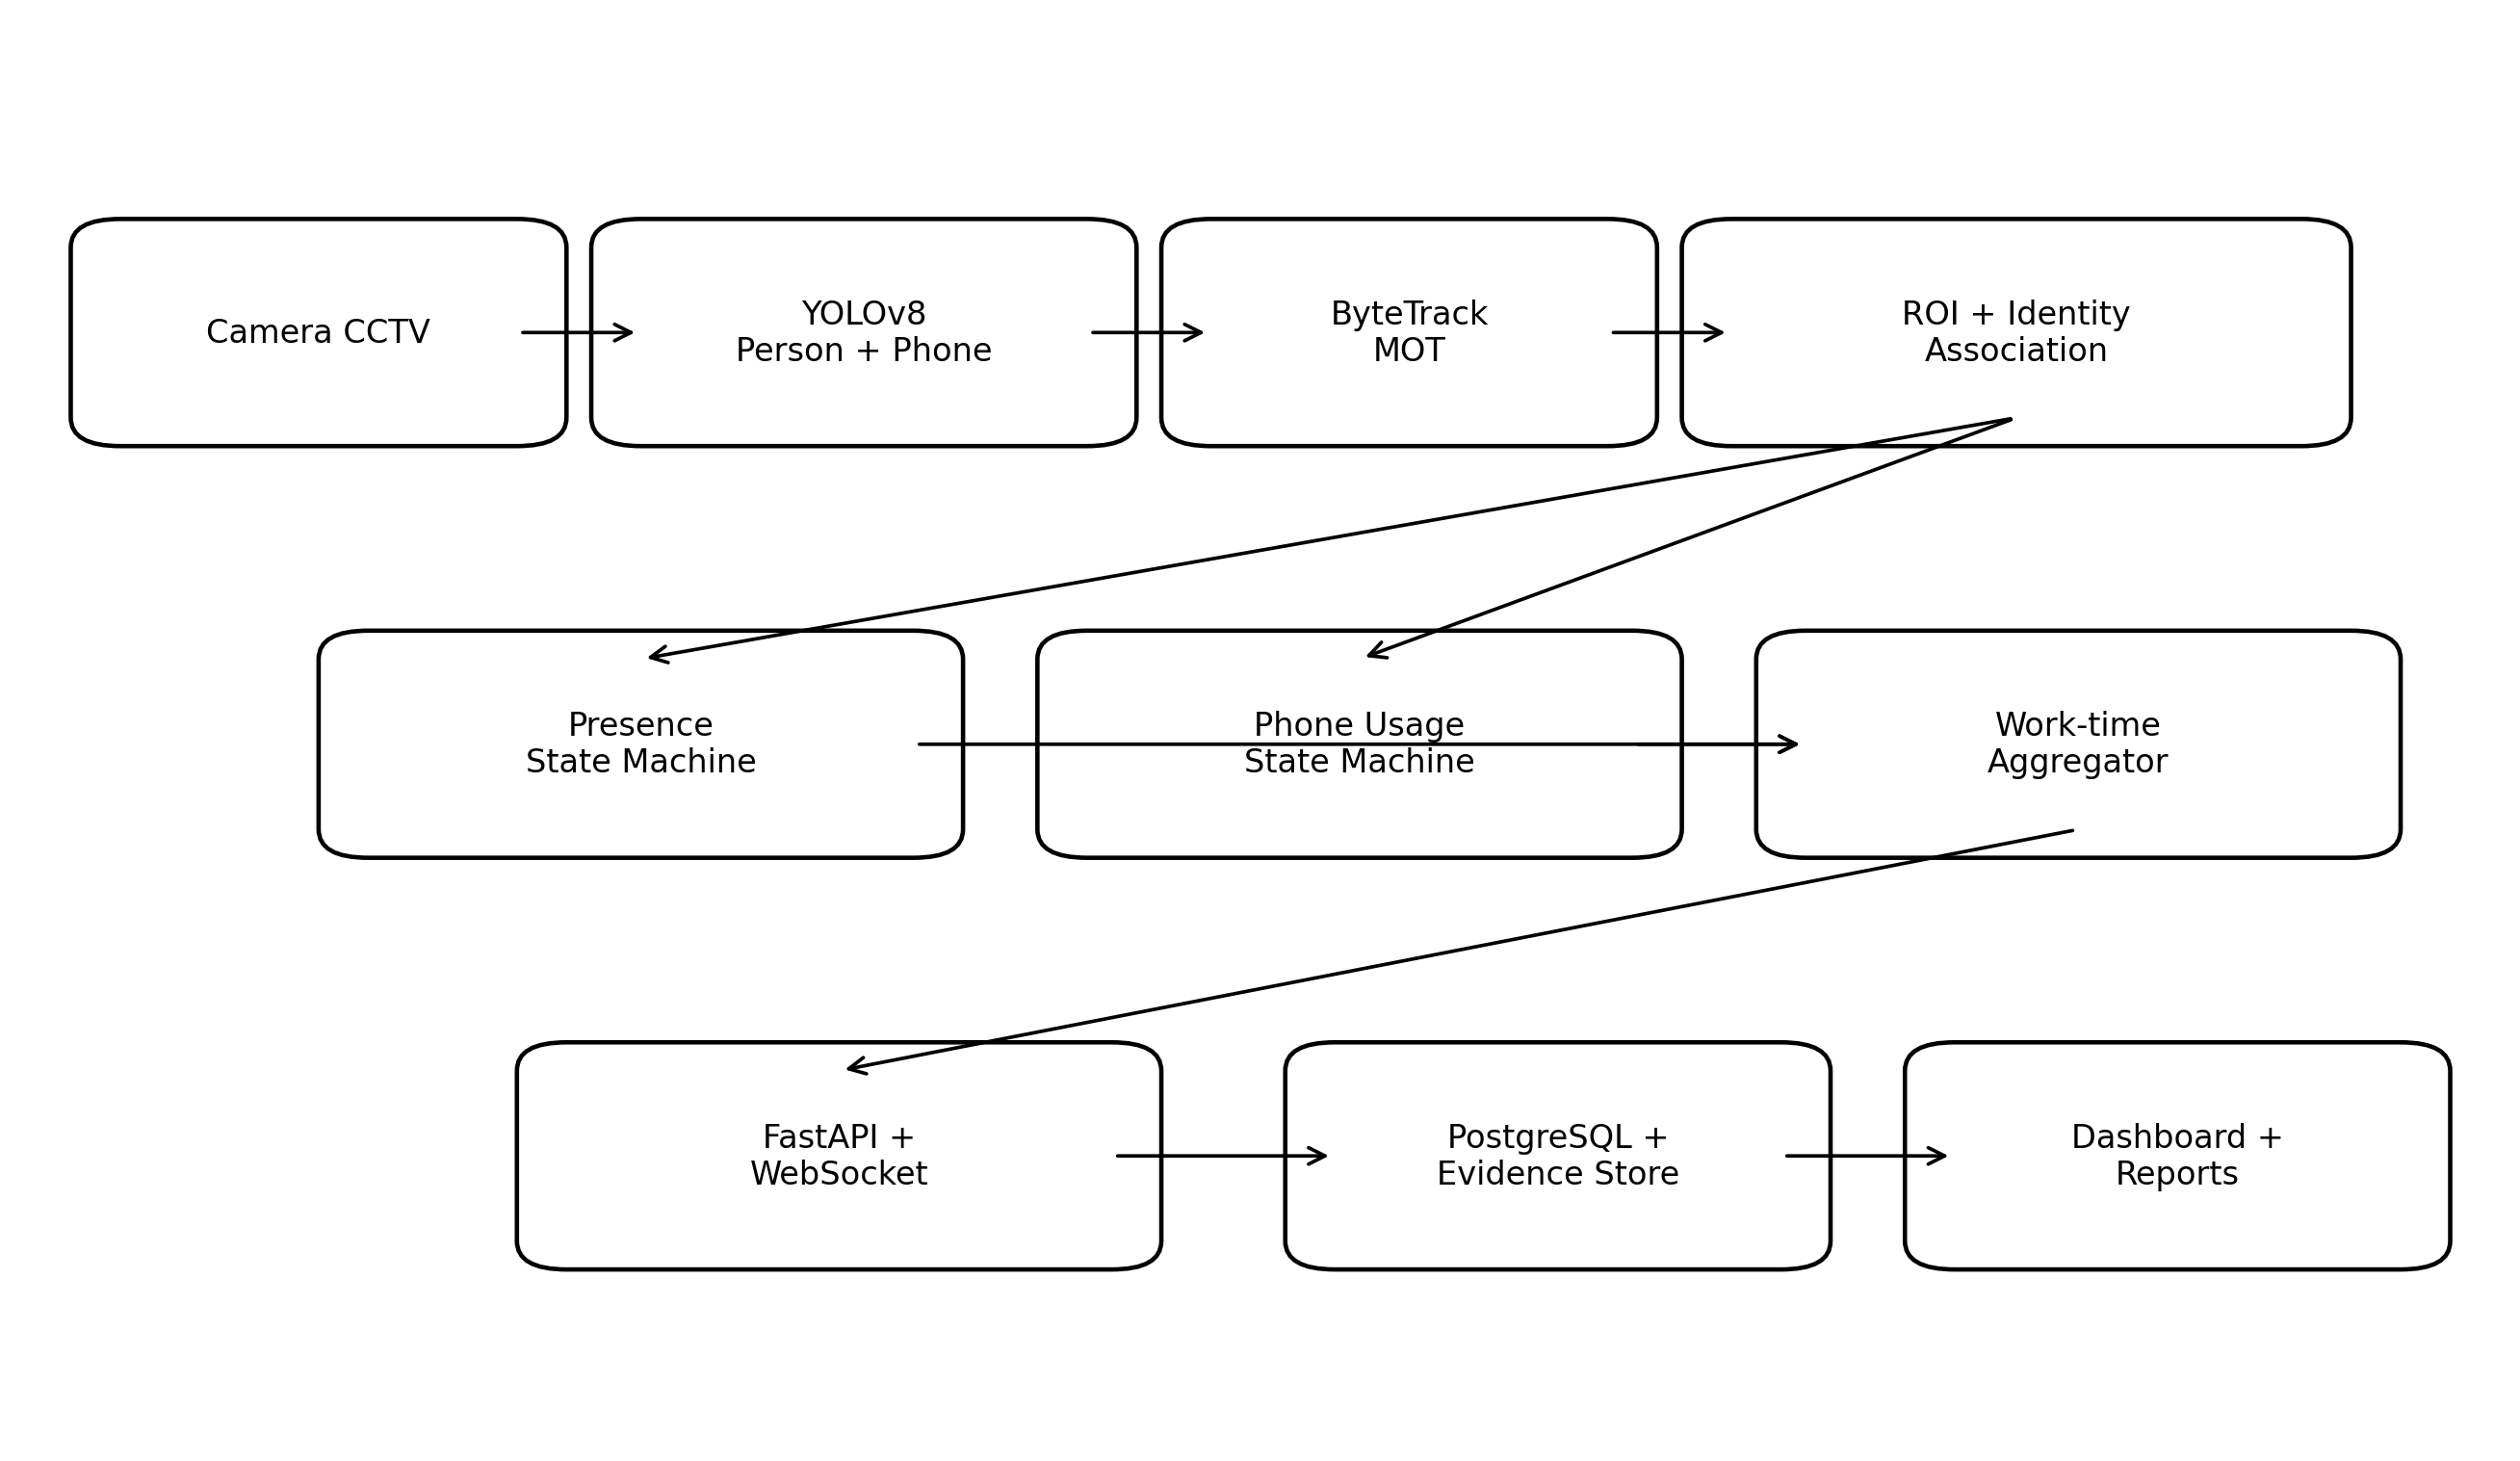
\includegraphics[width=0.98\textwidth]{Images/new_architecture.png}
\caption{Luồng xử lý đầu-cuối của hệ thống}
\label{fig:architecture-ch4}
\end{figure}

\subsection{Thiết kế pipeline thị giác máy tính}
\subsubsection{Thu nhận và chuẩn hóa frame}
Nguồn camera được trừu tượng hóa bởi \texttt{FrameSource}. Đối với RTSP, một thread đọc frame riêng giúp hạn chế việc vòng xử lý bị chặn khi network jitter. Mỗi frame mang theo timestamp monotonic cục bộ và timestamp wall-clock. Monotonic time dùng cho đo duration để tránh lỗi khi đồng hồ hệ thống thay đổi; wall-clock dùng cho báo cáo và đồng bộ với server.

Frame được resize giữ tỉ lệ về kích thước inference, ví dụ cạnh dài 640 pixel. Tọa độ detection sau đó được ánh xạ lại hệ tọa độ frame gốc để ROI và snapshot nhất quán. Nếu camera đổi resolution giữa phiên, client đánh dấu configuration mismatch thay vì âm thầm scale polygon theo một tỉ lệ không kiểm chứng.

\subsubsection{Detector dùng chung cho person và cell phone}
YOLO được gọi một lần cho mỗi frame được chọn xử lý. Đầu ra tách thành hai danh sách:
\begin{align}
 D^{person}_t &= \{d_i\mid class(d_i)=person\},\\
 D^{phone}_t &= \{d_i\mid class(d_i)=cell\ phone\}.
\end{align}
Ngưỡng confidence có thể khác nhau giữa hai lớp. Person cần ưu tiên recall để tracker không mất quỹ đạo, trong khi phone cần thận trọng hơn vì false positive có thể dẫn đến trừ thời gian. Tham số NMS/confidence được cấu hình tập trung và ghi vào metadata phiên để báo cáo có thể tái lập cấu hình.

\subsubsection{Theo dõi người bằng ByteTrack}
Tracker nhận $D^{person}_t$ và trả danh sách \texttt{TrackedPerson}. Mỗi phần tử gồm track ID, box, score, tuổi track, số frame đã thấy và trạng thái tracked/lost. ByteTrack được chọn theo phân tích Chương 2 vì cơ chế liên kết detection score thấp phù hợp che khuất ngắn \cite{bytetrack}.

Để tránh ID switch gây chuyển thời gian giữa nhân viên, hệ thống không gắn employee ngay khi track vừa sinh. Track cần đạt tuổi tối thiểu $N_{stable}$ hoặc presence candidate đủ lâu. Khi track bị lost dưới ngưỡng tracker buffer, association với vùng vẫn được giữ trong trạng thái GRACE nhưng không sinh detection mới.

\subsection{Thiết kế khu vực làm việc}
\subsubsection{Mô hình WorkArea}
Một WorkArea gồm: \texttt{id}, \texttt{camera\_id}, tên, polygon chuẩn hóa, trạng thái active và phiên bản cấu hình. Assignment giữa employee và area có \texttt{effective\_from}/\texttt{effective\_to}. Nhờ đó cùng một ROI có thể được gán cho nhân viên khác ở ca sau mà không sửa lịch sử cũ.

Polygon được lưu dạng các điểm $(u_i,v_i)\in[0,1]^2$. Khi frame có kích thước $(W,H)$, điểm thực tế là $(u_iW,v_iH)$. Client xác minh tối thiểu ba đỉnh và diện tích polygon lớn hơn ngưỡng; polygon lỗi không được kích hoạt.

\subsubsection{ROI matching}
Với mỗi track, tính anchor $p(q)$ theo công thức \ref{eq:anchor}. Nếu anchor nằm trong đúng một ROI, track được gán ứng viên cho vùng đó. Nếu không nằm vùng nào, \texttt{area\_id=None}. Nếu nằm nhiều vùng do polygon chồng lấn, score vùng:
\begin{equation}
 S_{area}=\lambda_1 S_{inside}+\lambda_2 S_{center}+\lambda_3 S_{history},
\end{equation}
trong đó $S_{history}$ ưu tiên vùng trước đó để tạo hysteresis không gian. Thiết kế yêu cầu giao diện cảnh báo khi hai polygon chồng lấn lớn vì đây là cấu hình nên tránh.

\begin{figure}[H]
\centering
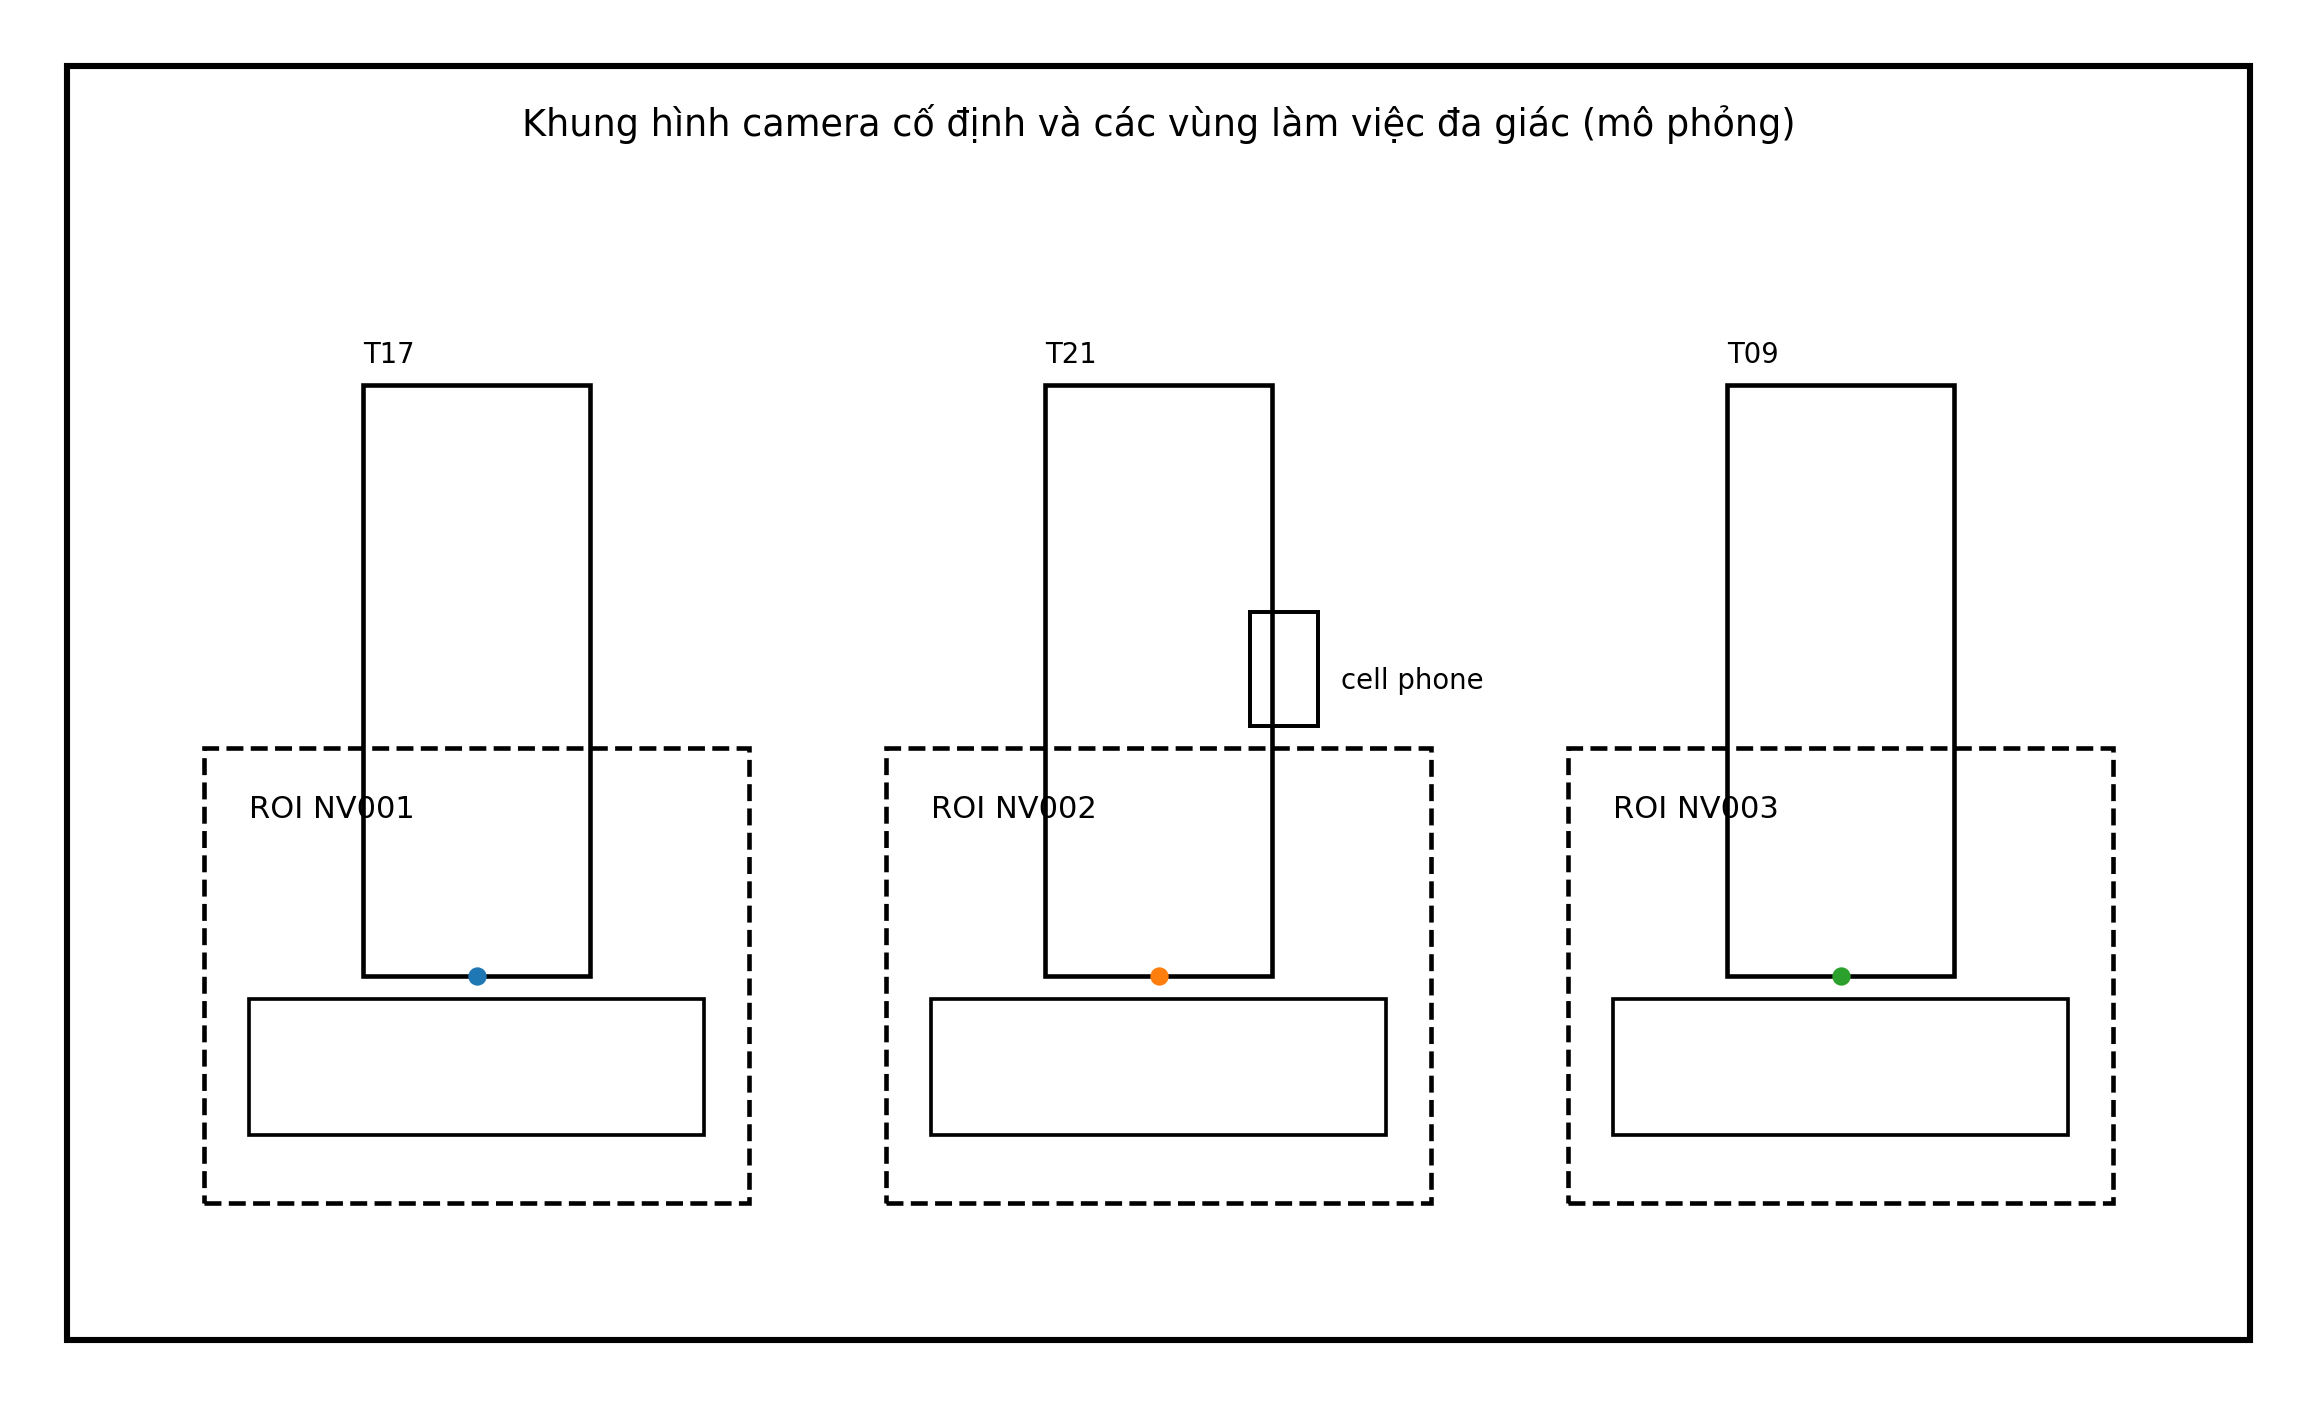
\includegraphics[width=0.94\textwidth]{Images/roi_scene.png}
\caption{Minh họa ánh xạ track người vào vùng làm việc}
\label{fig:roi-ch4}
\end{figure}

\subsection{Thiết kế liên kết danh tính}
\subsubsection{Hồ sơ EmployeeIdentity}
Mỗi nhân viên có nhiều embedding tham chiếu thay vì một vector duy nhất. Enrollment lấy ảnh mặt ở vài góc vừa phải, chạy face detector/crop, chuẩn hóa rồi tạo embedding. Vector có thể lưu dưới dạng mảng float đã mã hóa và được bảo vệ quyền riêng biệt. Để giảm nhiễu, có thể lưu centroid và các vector mẫu.

\subsubsection{Kích hoạt xác minh theo sự kiện}
Face verification không chạy mọi frame. Scheduler kích hoạt khi: track mới đã ổn định; track nằm trong area có employee assignment nhưng chưa verified; đến chu kỳ recheck; hoặc có sự kiện nghi ngờ như track mới thay thế track cũ ngay sau absence. Giới hạn tần suất giúp GPU tập trung cho detector/tracker.

\subsubsection{Quy tắc quyết định}
Giả sử $s$ là similarity tốt nhất giữa embedding track và hồ sơ employee. Dùng hai ngưỡng $\theta_{verify}>\theta_{reject}$:
\begin{itemize}
\item $s\geq\theta_{verify}$ và đủ số mẫu: VERIFIED.
\item $s<\theta_{reject}$ lặp lại đủ $k$ lần: MISMATCH.
\item khoảng giữa hoặc thiếu mặt: UNKNOWN/PROVISIONAL.
\end{itemize}
Hai ngưỡng tạo margin thay vì ép nhãn ở vùng không chắc chắn. Giá trị cụ thể phải tune trên dữ liệu thật; trong cấu hình mô phỏng có thể dùng 0.65/0.50 chỉ để kiểm thử luồng, không xem là threshold tối ưu.

\subsection{Máy trạng thái hiện diện}
\subsubsection{Các trạng thái}
FSM hiện diện gồm:
\begin{enumerate}
\item \textbf{ABSENT}: không có track hợp lệ trong vùng.
\item \textbf{CANDIDATE}: bắt đầu có track ứng viên nhưng chưa đủ thời lượng xác nhận.
\item \textbf{PRESENT}: hiện diện đã xác nhận.
\item \textbf{GRACE}: track vừa mất hoặc tạm ra khỏi điều kiện, đang chờ trước khi kết luận vắng.
\end{enumerate}

\begin{figure}[H]
\centering
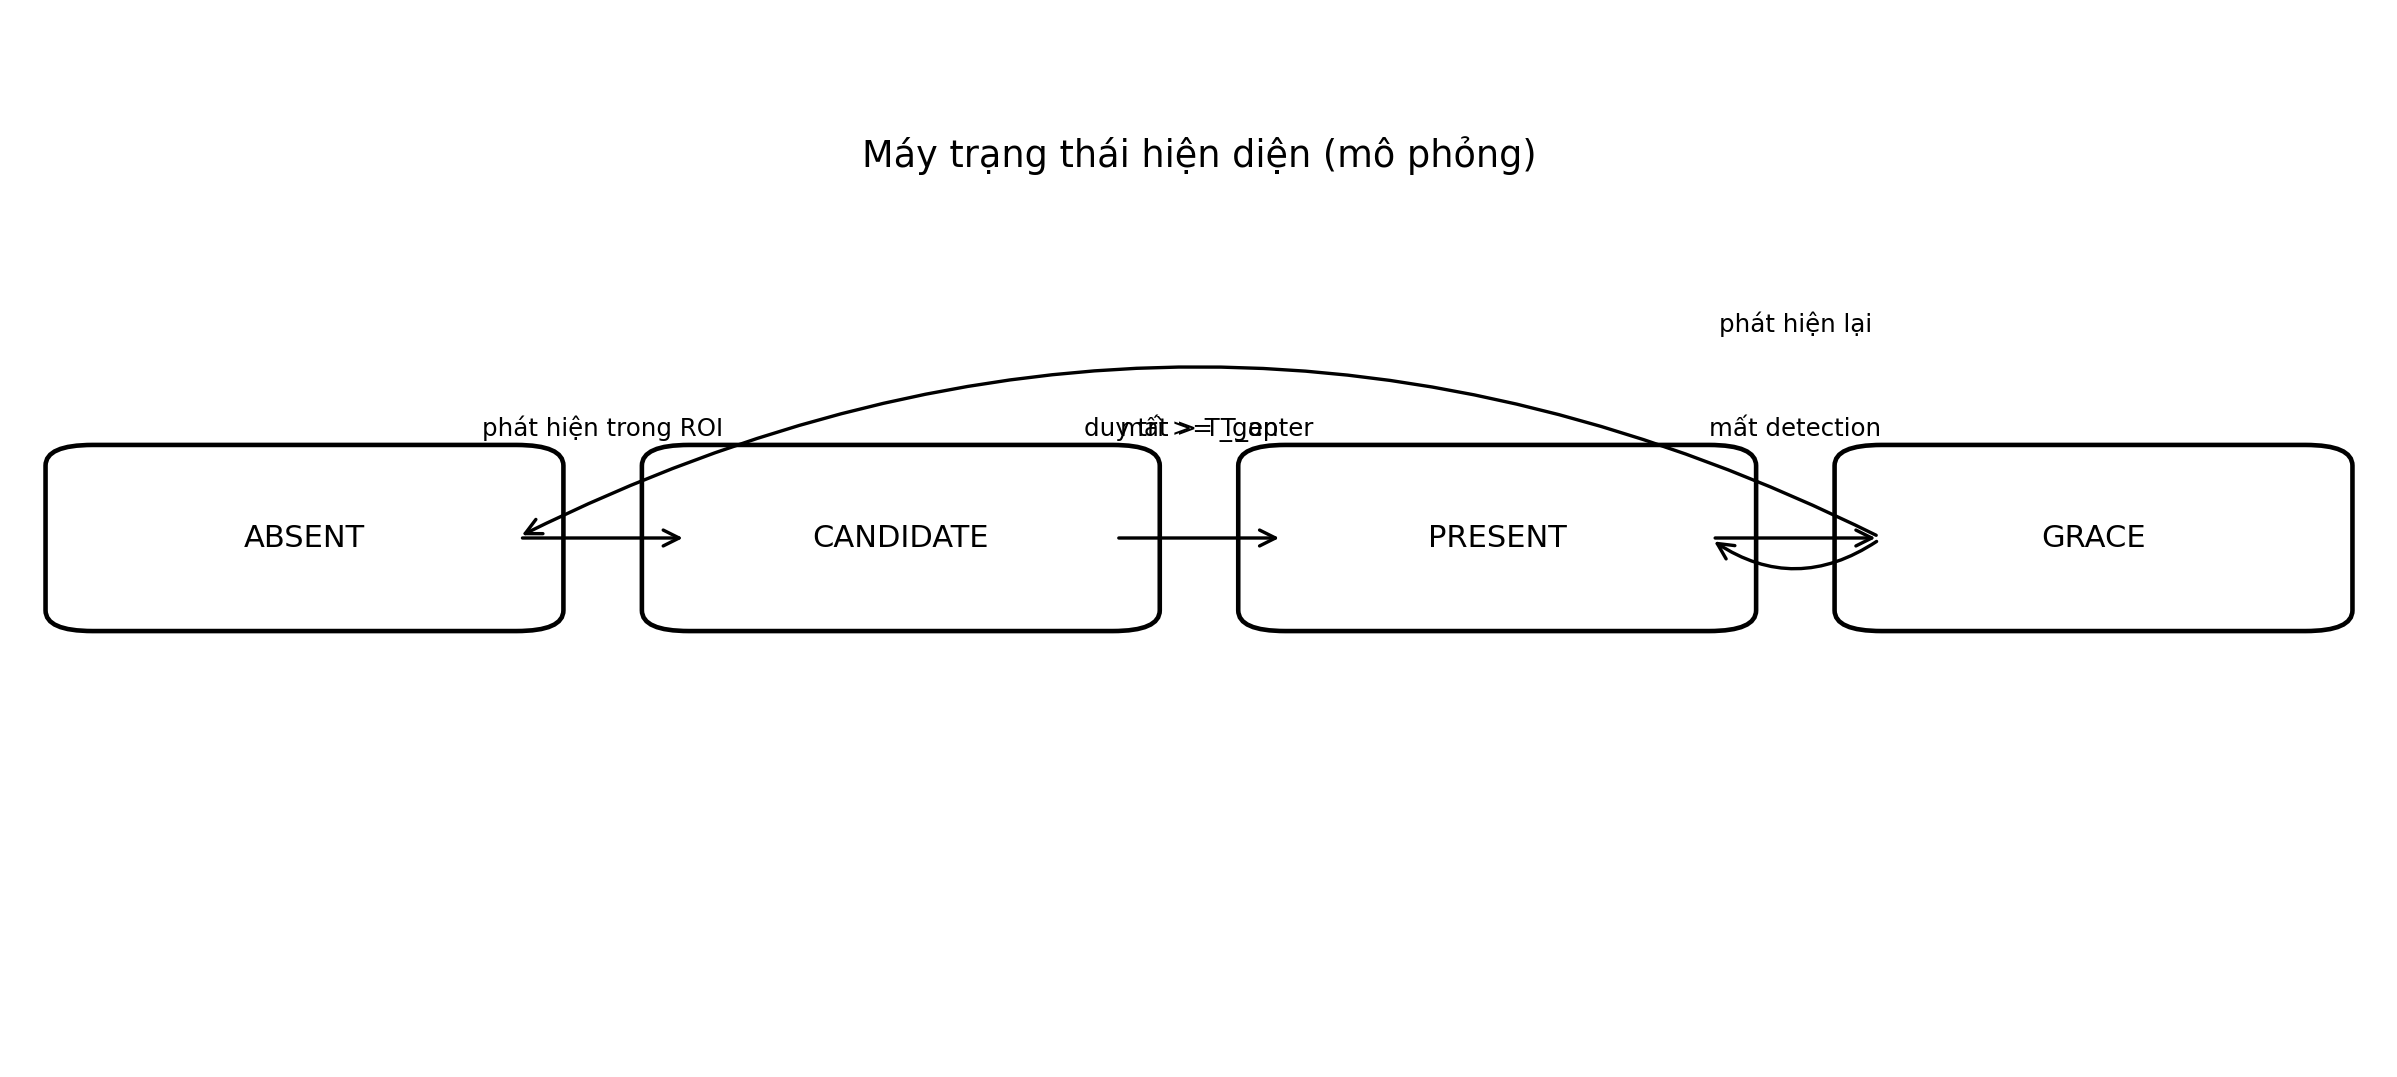
\includegraphics[width=0.95\textwidth]{Images/presence_state.png}
\caption{Máy trạng thái hiện diện ở cấp nhân viên}
\label{fig:presence-state-ch4}
\end{figure}

\subsubsection{Điều kiện chuyển}
Từ ABSENT sang CANDIDATE khi có track phù hợp area và identity không MISMATCH. CANDIDATE sang PRESENT khi tồn tại đủ $T_{enter}$ và tỉ lệ quan sát hợp lệ vượt $r_{enter}$. Nếu ứng viên biến mất trước ngưỡng thì trở về ABSENT mà không tạo interval.

PRESENT sang GRACE khi không còn detection phù hợp. Nếu track trở lại trong $T_{gap}$ thì quay PRESENT, interval không bị cắt. Nếu quá $T_{gap}$ thì chuyển ABSENT và đóng interval tại \texttt{last\_confirmed\_seen}, không phải tại thời điểm hết grace. Đây là chi tiết quan trọng để không cộng dư $T_{gap}$ mỗi lần nhân viên rời đi.

\subsubsection{Xử lý dữ liệu không hợp lệ}
Nếu camera frame lỗi, model exception hoặc latency quá ngưỡng, trạng thái quan sát là UNKNOWN thay vì ABSENT. Timer absence không tăng trong khoảng dữ liệu không đáng tin cậy quá ngắn. Nếu camera mất lâu hơn timeout hệ thống, phiên được đánh dấu CAMERA\_OFFLINE; thời gian này không được tự động coi là absent/present và báo cáo tách riêng \textit{unobserved duration}.

\subsection{Thiết kế nhận biết sử dụng điện thoại}
\subsubsection{Phone--person association}
Mỗi phone detection được so với các tracked person đang active. Interaction region được tạo từ person box bằng cách mở rộng phần thân trên theo tỉ lệ cấu hình. Score theo công thức \ref{eq:phoneassoc} gồm khoảng cách, containment và ROI consistency. Mỗi phone chỉ được gán tối đa cho một person và mỗi person có thể nhận phone tốt nhất trong frame.

Nếu score tốt nhất dưới $\theta_{assoc}$ hoặc chênh lệch giữa hai person tốt nhất nhỏ hơn margin $\Delta$, association là UNKNOWN. Quy tắc này ưu tiên bỏ qua trường hợp mơ hồ hơn là gán sai người, vì WPAR là chỉ số rủi ro trực tiếp.

\subsubsection{Máy trạng thái phone}
FSM gồm NO\_PHONE, CANDIDATE, USING, GRACE. Detection liên kết phải duy trì $T_{phone\_enter}$ để vào USING. Khi mất phone, GRACE kéo dài $T_{phone\_exit}$ nhằm hấp thụ che tay ngắn. Nếu hết grace, phiên kết thúc tại last-associated timestamp.

\begin{figure}[H]
\centering
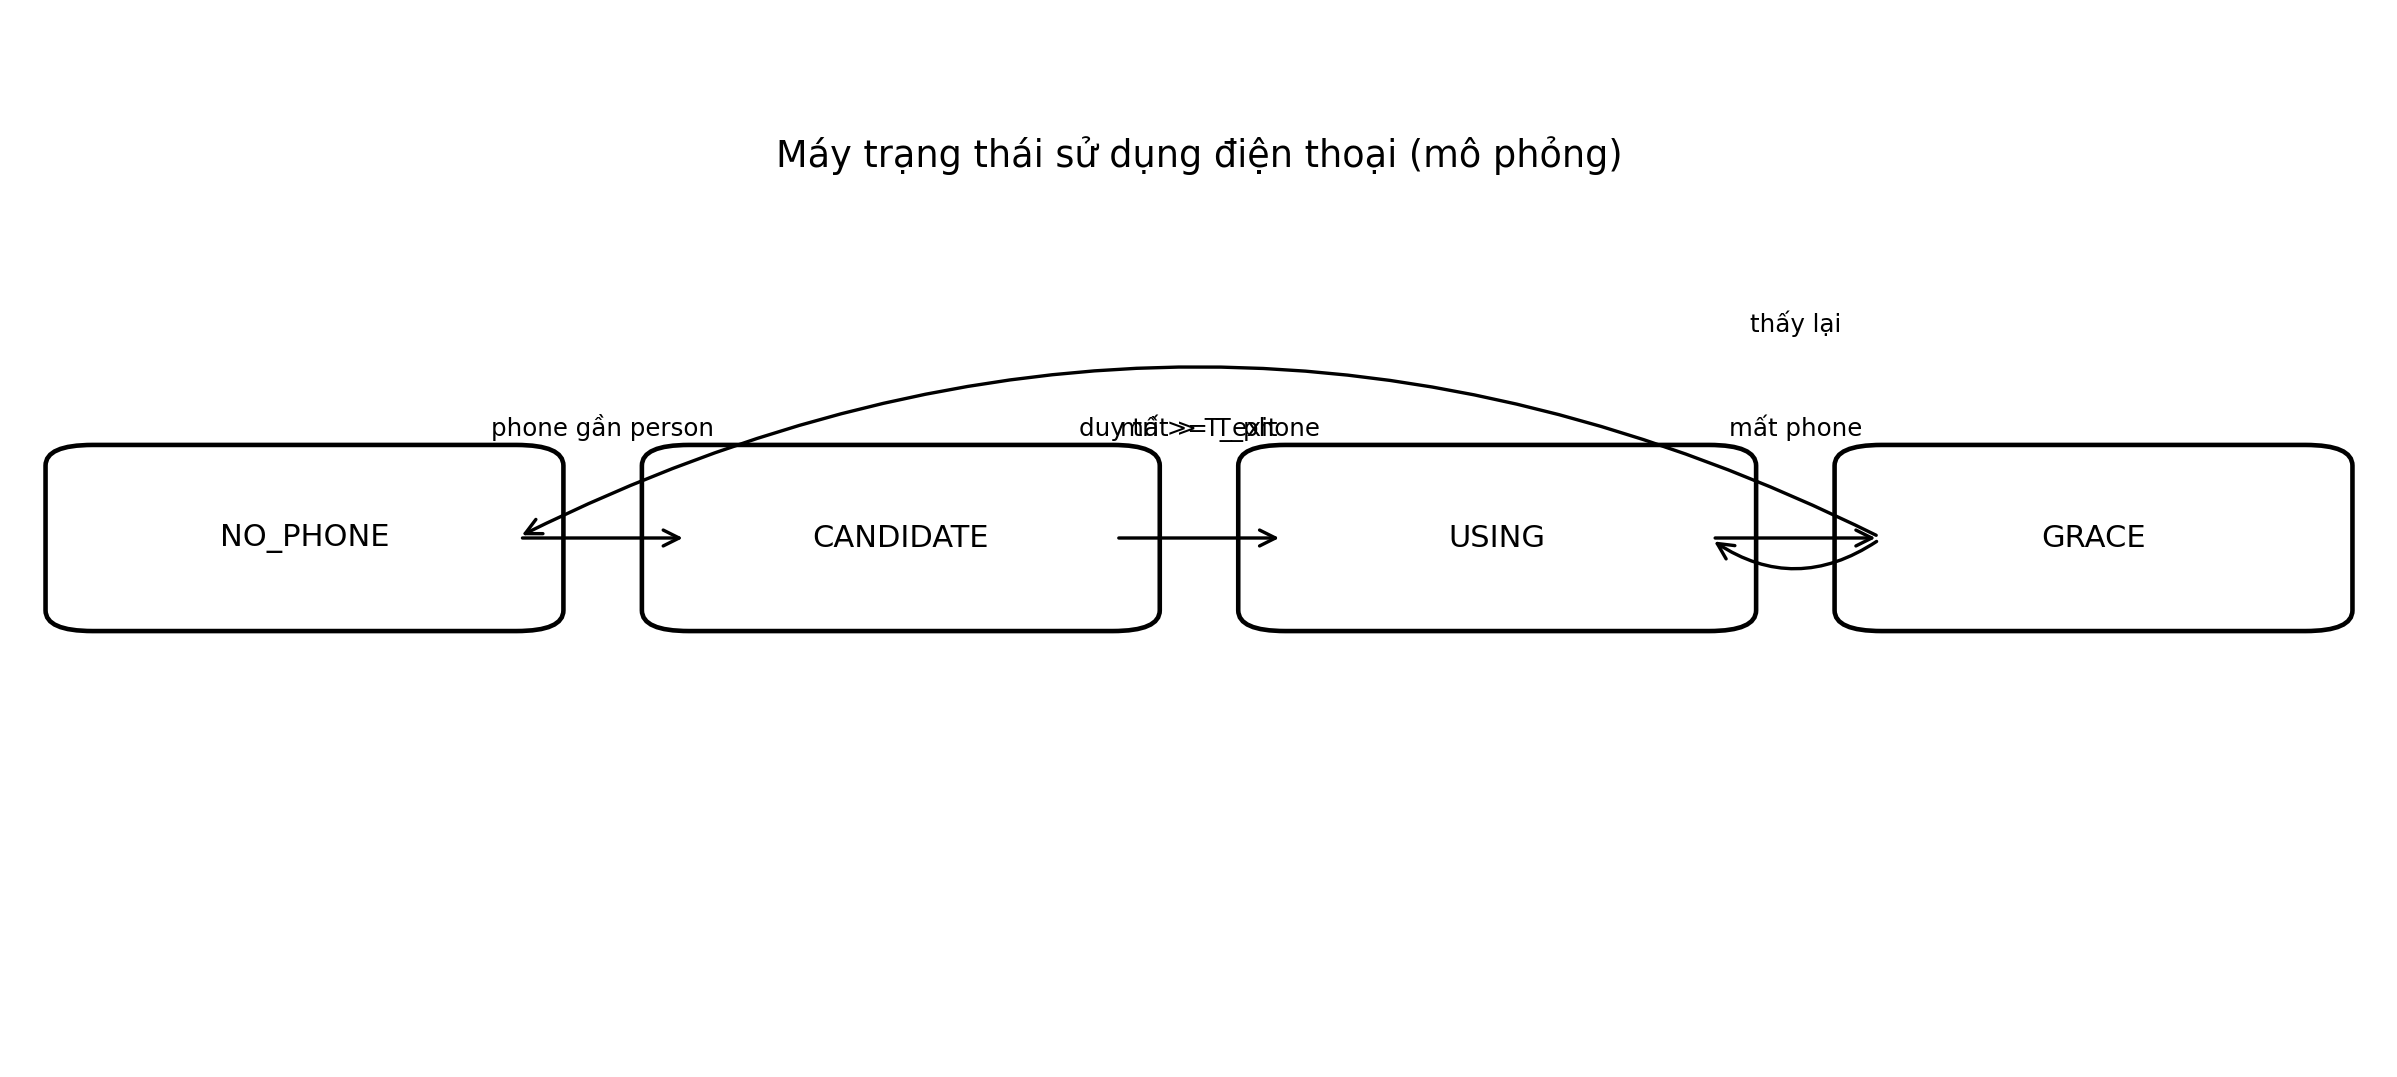
\includegraphics[width=0.95\textwidth]{Images/phone_state.png}
\caption{Máy trạng thái theo dõi phiên sử dụng điện thoại}
\label{fig:phone-state-ch4}
\end{figure}

\subsubsection{Không tính phone khi không hiện diện}
Phone state phụ thuộc presence. Nếu employee không PRESENT, phone detection trong ROI không tạo phone session cho employee đó. Khi presence chuyển ABSENT, phone session đang mở được đóng ở thời điểm last present. Quy tắc này tránh double deduction giữa absence và phone.

\subsection{Bộ tổng hợp thời gian làm việc}
\subsubsection{Mô hình dữ liệu interval}
\texttt{PresenceInterval} gồm employee, area, start/end, confidence aggregate, identity state và reason đóng. \texttt{PhoneUsageInterval} gồm employee, track, start/end, confidence và evidence ref. Interval chưa đóng được lưu current state; khi đóng mới trở thành bản ghi bền vững hoặc event materialized.

\subsubsection{Tính theo ca}
Giả sử lịch làm việc gồm hai cửa sổ $W_1=[08{:}00,12{:}00]$, $W_2=[13{:}00,17{:}30]$. Aggregator lấy giao mọi presence interval với $W_1\cup W_2$, nhờ đó thời gian nghỉ trưa ngoài cửa sổ không cần suy luận từ camera. Nếu ca qua đêm, cửa sổ được biểu diễn bằng timestamp tuyệt đối thay vì chỉ giờ trong ngày.

\subsubsection{Chính sách điện thoại}
Policy có dạng:
\begin{Verbatim}[fontsize=\small,breaklines=true,breakanywhere=true]
phone_usage:
  enabled: true
  allowance_minutes_per_shift: 15
  min_session_seconds: 3
  deduction_enabled: true
  evidence_on_start: false
  evidence_on_excess: true
\end{Verbatim}
Khi tổng phone chưa vượt allowance, effective time bằng presence. Khi vượt, chỉ phần excess trừ theo phương trình \ref{eq:effective}. Policy version được gắn vào summary để về sau biết phép tính sử dụng quy định nào.

\subsubsection{Ví dụ tính toán}
Một nhân viên có $T_{presence}=7$ giờ $45$ phút, $T_{phone}=32$ phút và allowance 15 phút. Khi đó $T_{excess}=17$ phút và $T_{effective}=7$ giờ $28$ phút. Nếu deduction bị tắt, hệ thống vẫn hiển thị phone 32 phút nhưng effective không bị trừ. Tách measurement và policy giúp tránh việc CV quyết định trực tiếp quy định nhân sự.

\subsection{Thiết kế giao tiếp thời gian thực}
\subsubsection{Telemetry camera}
Camera gửi snapshot trạng thái theo chu kỳ, ví dụ 1 giây, thay vì mọi frame. Schema logic:
\begin{Verbatim}[fontsize=\small,breaklines=true,breakanywhere=true]
CameraTelemetry {
  camera_id, sequence, captured_at,
  fps, pipeline_latency_ms,
  persons: [
    {track_id, bbox, employee_id?, area_id?,
     identity_state, presence_state,
     phone_state, confidence}
  ]
}
\end{Verbatim}
Server không cần lưu toàn bộ telemetry dài hạn; current state được cập nhật để dashboard hiển thị.

\subsubsection{Event}
Event chỉ sinh ở transition có ý nghĩa: PRESENCE\_CONFIRMED, ABSENCE\_CONFIRMED, PHONE\_START, PHONE\_END, PHONE\_EXCESS\_REACHED, IDENTITY\_VERIFIED, IDENTITY\_MISMATCH, CAMERA\_OFFLINE/ONLINE. Event có ID duy nhất để client retry mà server vẫn idempotent.

\subsubsection{Timestamp và sequence}
Server dùng received timestamp để kiểm tra lệch đồng hồ nhưng giữ captured timestamp cho duration. Sequence tăng dần trong mỗi camera session. Nếu message đến lộn thứ tự, server không áp dụng current state cũ hơn. Khi reconnect, client có thể gửi event queue còn thiếu theo event ID.

\subsection{Thiết kế mô hình dữ liệu}
Các thực thể chính:
\begin{itemize}
\item \texttt{Organization}, \texttt{User}, \texttt{OrganizationMembership}, \texttt{AuditLog}: kế thừa hạ tầng quản trị.
\item \texttt{Employee}: hồ sơ nhân viên không bắt buộc là tài khoản đăng nhập.
\item \texttt{EmployeeIdentity}: face embedding và metadata enrollment.
\item \texttt{Camera}: nguồn CCTV, trạng thái, cấu hình và version.
\item \texttt{WorkArea}: polygon ROI thuộc camera.
\item \texttt{EmployeeWorkAreaAssignment}: ánh xạ theo thời gian.
\item \texttt{WorkSchedule}: ca làm và khoảng nghỉ.
\item \texttt{MonitoringSession}: vòng đời client camera.
\item \texttt{PresenceInterval}, \texttt{PhoneUsageInterval}: dữ liệu thời gian.
\item \texttt{DailyWorkSummary}: snapshot tổng hợp cuối ngày.
\item \texttt{Evidence}, \texttt{Review}, \texttt{ReportJob}: hậu kiểm và báo cáo.
\end{itemize}

\begin{table}[H]
\centering
\caption{Các trường cốt lõi của DailyWorkSummary}
\label{tab:summary-fields}
\begin{tabularx}{\textwidth}{p{4.4cm}p{3.3cm}X}
\toprule
\textbf{Trường} & \textbf{Kiểu} & \textbf{Ý nghĩa}\\
\midrule
employee\_id & UUID/FK & Nhân viên\\
date & Date & Ngày tổng hợp\\
gross\_presence\_sec & Integer & Tổng hiện diện trong lịch làm\\
phone\_usage\_sec & Integer & Tổng phone session hợp lệ\\
phone\_allowance\_sec & Integer & Hạn mức theo policy version\\
excess\_phone\_sec & Integer & Phần vượt mức\\
effective\_work\_sec & Integer & Giá trị sau điều chỉnh\\
unobserved\_sec & Integer & Thời gian camera không đủ dữ liệu\\
policy\_version & String & Phiên bản quy tắc tính\\
\bottomrule
\end{tabularx}
\end{table}

\subsection{Thiết kế phân quyền và bảo vệ dữ liệu}
Authorization được kiểm tra theo tổ chức và resource. Organization Admin có thể quản lý employee/camera/policy; Supervisor chỉ xem camera/nhân viên được gán. Quyền xem face embedding không cấp trực tiếp qua API thông thường; chỉ service identity có quyền đọc dữ liệu cần thiết. Snapshot evidence yêu cầu permission riêng và đường dẫn file không được lấy trực tiếp từ input client.

Camera dùng token loại riêng, không dùng JWT người dùng. Token camera gắn camera ID, organization ID và version thu hồi. WebSocket dashboard dùng ticket ngắn hạn một lần để tránh đặt bearer token trong URL. Ảnh evidence kiểm tra MIME/magic bytes, giới hạn kích thước và tên file do server sinh.

Retention policy tách metadata tổng hợp và ảnh. Summary có thể lưu lâu hơn; snapshot có thời gian ngắn hơn và tự xóa theo job. Audit ghi ai xem/tải evidence. Các quyết định này phù hợp nguyên tắc giảm thiểu dữ liệu và kiểm soát truy cập nêu ở Chương 2.

\subsection{Luồng nghiệp vụ đầu-cuối}
Một phiên hoạt động theo trình tự: client xác thực camera; tải configuration version; mở nguồn video; chạy preflight; gửi CAMERA\_ONLINE; bắt đầu telemetry. Khi employee vào ROI, presence state chuyển; identity verifier có thể chạy; transition được gửi event. Phone session xử lý song song. Cuối ca hoặc khi dừng camera, client đóng interval mở, gửi SESSION\_END; server chạy materializer để bảo đảm interval/summary nhất quán; reporting worker sinh báo cáo.

Nếu mạng mất, client tiếp tục trạng thái cục bộ và queue event. Current dashboard chuyển camera sang disconnected theo heartbeat timeout. Khi mạng trở lại, event chưa ACK được gửi lại với event ID cũ. Server dùng idempotency key tránh tạo interval trùng.

\subsection{Khả năng giải thích và hậu kiểm}
Mọi con số trong báo cáo phải truy về interval/event. Khi effective thấp do phone excess, giao diện hiển thị gross presence, allowance, các phone session và evidence tương ứng. Khi identity UNKNOWN kéo dài, summary đánh cờ \textit{needs review} thay vì tự động trừ. Người quản lý có thể ghi review độc lập; raw event không bị sửa để bảo toàn audit trail.

\subsection{Các quyết định thiết kế đáng chú ý}
\begin{table}[H]
\centering
\caption{Các quyết định kiến trúc và lý do}
\label{tab:design-decisions}
\begin{tabularx}{\textwidth}{p{4.2cm}X X}
\toprule
\textbf{Quyết định} & \textbf{Lý do} & \textbf{Đánh đổi}\\
\midrule
Một YOLO cho person+phone & Chia sẻ inference, giảm tải & Hai lớp có thể cần threshold khác\\
ByteTrack thay detector-frame-only & Duy trì quỹ đạo, giảm đứt interval & Có nguy cơ ID switch\\
ROI là tín hiệu chính, face là hỗ trợ & Camera xa không luôn thấy mặt & Cần quản lý assignment chính xác\\
FSM và backdating interval & Lọc nhiễu nhưng giảm bias thời gian & Logic phức tạp hơn if-else\\
Phone association bảo thủ & Giảm trừ nhầm người & Có thể bỏ sót phiên mơ hồ\\
SQL current + event store & Dashboard nhanh và vẫn truy vết & Hai lớp lưu trữ cần đồng bộ\\
Không truyền video liên tục & Giảm băng thông/quyền riêng tư & Dashboard không xem live video đầy đủ\\
\bottomrule
\end{tabularx}
\end{table}

\subsection{Kết luận chương}
Thiết kế tập trung vào việc bảo toàn ý nghĩa theo thời gian: detection được biến thành track; track được đặt trong ngữ cảnh ROI/identity; quan sát được biến thành state; state được biến thành interval; interval được tổng hợp thành thời gian và mọi điều chỉnh bởi phone policy vẫn truy vết được. Đây là chuỗi logic chính cần được phản ánh nhất quán trong cài đặt và đánh giá.
